\begin{frame}[c]{}

\centering
\huge
Lecture 3:\\
Evaluation and Visualization
\end{frame}
%----------------------------------------------------------------------
%----------------------------------------------------------------------
\begin{frame}[c]{Where are we? The big picture}

\begin{itemize}
	\item Introduction
	\item[$\to$] Background
	\begin{itemize}
		\item Design spaces in ML
		\item[$\to$] Evaluation and visualization
	\end{itemize}
	\item Hyperparameter optimization (HPO)
	\begin{itemize}
	  \item Bayesian optimization
	  \item Other black-box techniques
	  \item Speeding up HPO with multi-fidelity optimization
	\end{itemize}
	\item Pentecost (Holiday) -- no lecture
	\item Architecture search I + II
	\item Meta-Learning
	\item Learning to learn $\&$ optimize
	\item Beyond AutoML: algorithm configuration and control
	\item Project announcement and closing
\end{itemize}


\end{frame}
%----------------------------------------------------------------------
%----------------------------------------------------------------------
\begin{frame}[c]{Learning Goals}

After this lecture, you will be able to \ldots

\begin{itemize}
	\item explain the role of outliers in CS/ML
	\item compare and visualize the performance of different configurations
	\item compare and visualize the performance of AutoML systems
	\item explain and correctly apply statistical hypothesis tests
\end{itemize}

\end{frame}
%----------------------------------------------------------------------

%----------------------------------------------------------------------
\begin{frame}[c]{How CS differs from other empirical sciences}

\begin{itemize}
	\item We have a complete and precise \alert{mathematical description}\\of the object under study
	\smallskip
	
	\item We have complete and precise \alert{control} of the object under study\\ 
	(and to some degree also the experimental environment)
	\begin{itemize}
		\item as a result, experiments can be \alert{reproduced perfectly}
		\pause
		\item what do we need for experiments to be reproducible? 
		\only<2-2>{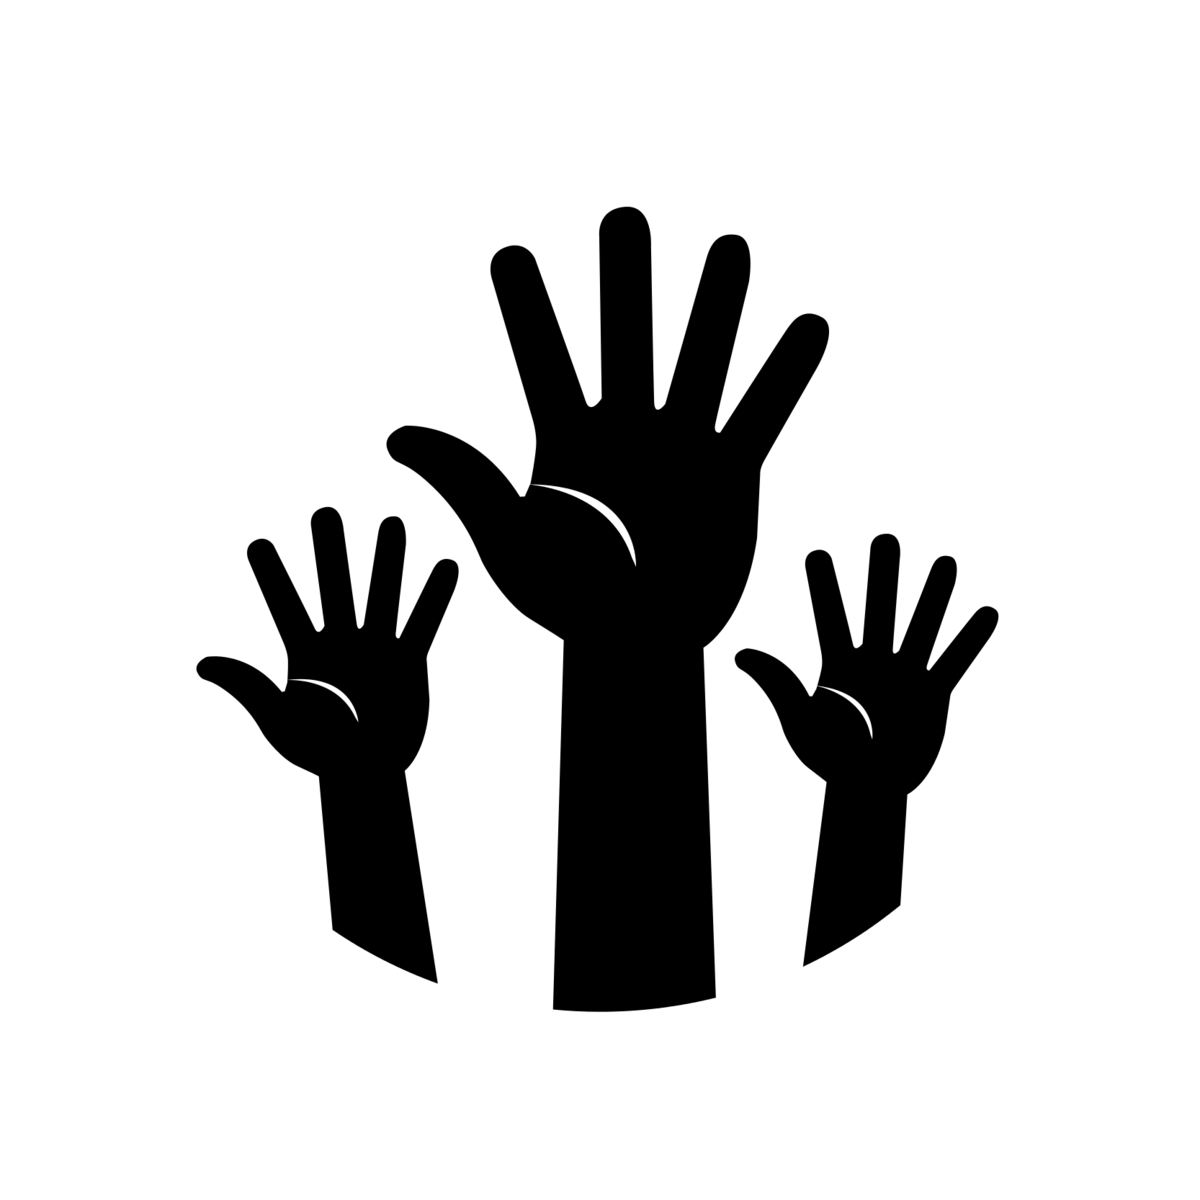
\includegraphics[height=1.5em]{images/hands}
		}
		\only<3->{
			\begin{itemize}
				\item  {Code \& dependencies, inputs, environment ($\rightarrow$ VM \& cloud)}
			\end{itemize}
			\pause
		}
	\end{itemize}
	\medskip
	\pause
	
	%\only<4->{
	\item We often have quite \alert{cheap} experiments
	\begin{itemize}
		\item price for computers is monotonically decreasing
		\item often maximal runtimes of 1h; exception: deep learning (up to a week)
		\item compare e.g., experimental physics: 1 week of beam time per year % Still different from observing new species in the field for half a year / 
	\end{itemize}
	\smallskip
	\pause
	%}
	%\only<5->{
	\item We can conduct and analyze experiments fully \alert{automatically} 
	\begin{itemize}
		\item we can gather large amounts of data quickly (e.g., 100 repetitions)
		\item but: don't confuse statistical significance and relevance
	\end{itemize}
	%}	
\end{itemize}

\end{frame}
%-----------------------------------------------------------------------
%----------------------------------------------------------------------
\begin{frame}[c]{Outliers are quite different in computer experiments}

Is the following statement correct? 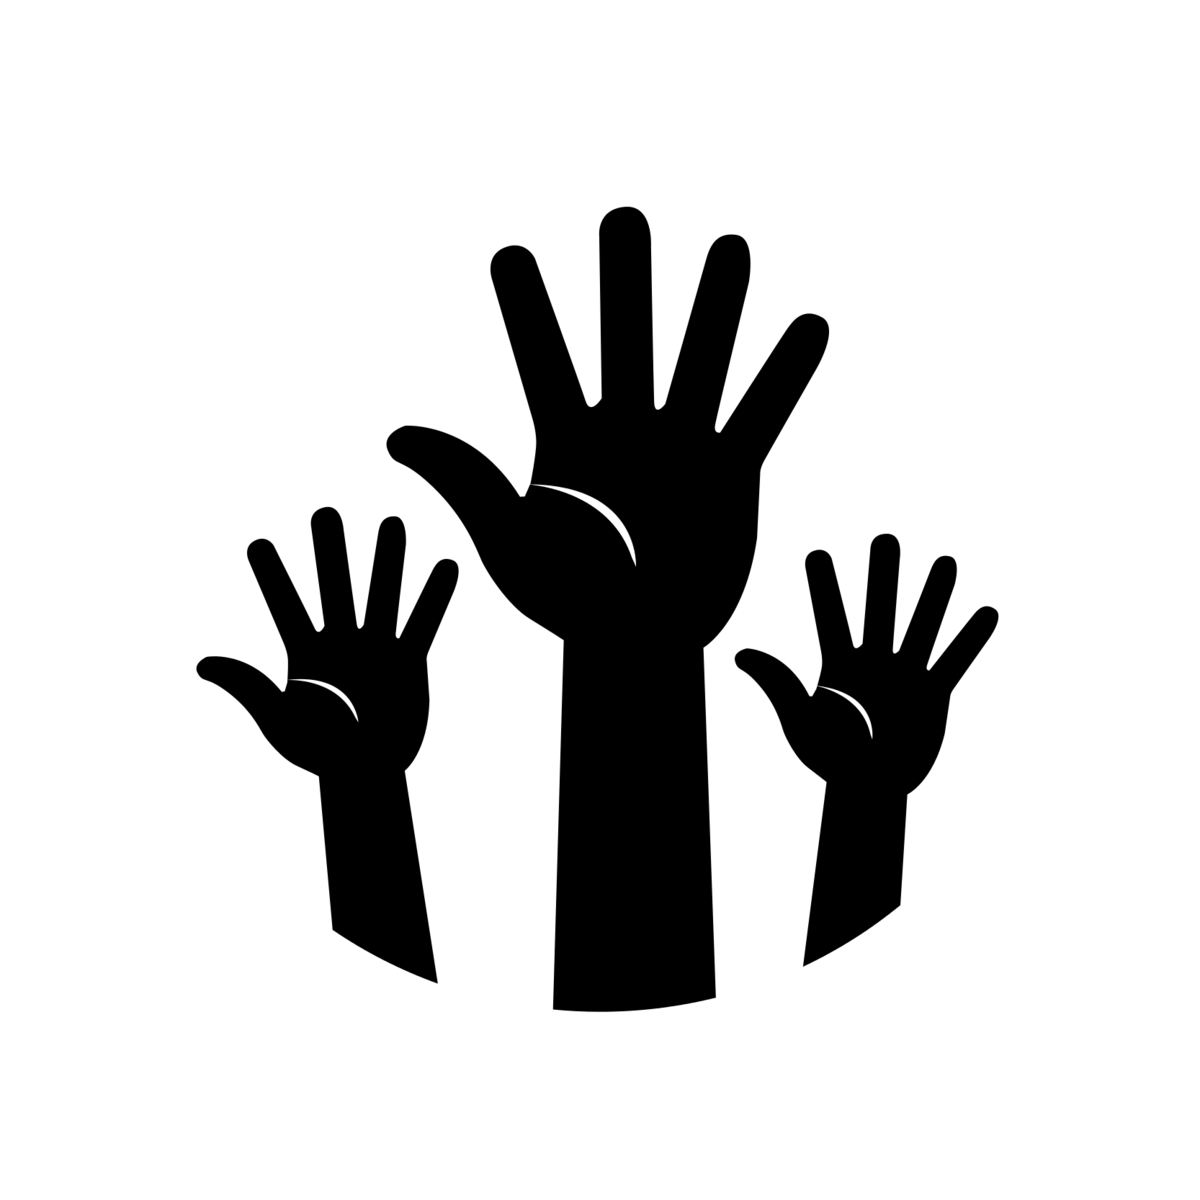
\includegraphics[height=1.5em]{images/hands}

``As usual in other empirical sciences, we (in CS) should take care to \alert{detect and remove outliers} before further analysis.''

\pause
\bigskip

\begin{block}{Outliers in CS/ML}
\begin{itemize}
	\item outliers should be investigated closely -- why is there an outlier?
	\item outliers are (hopefully) reproducible -- narrow down their reason!
	\pause
	\begin{itemize}
		\item \textbf{Algorithm:} When characterizing performance of an optimization algorithm, \alert{outliers with poor values can indicate (deep) local optima}
		\pause
		\item \textbf{Environment:} Outliers can indicate a \alert{problem with the environment} (e.g., file system or network issues)
		\pause
		\item \textbf{Datasets:}  When characterizing cost across a distribution of datasets, outliers with small values can indicate trivial datasets.
	\end{itemize}
\end{itemize}
\end{block}

\end{frame}
%-----------------------------------------------------------------------
\section{Visualization of Configuration Performance}
%----------------------------------------------------------------------
%----------------------------------------------------------------------
\begin{frame}[c]{Setup}

For the following slides, we have used the following setup:

\begin{itemize}
	\item Model: simple MLP (from sklearn)\\ with 2 layers with 128 neurons and 64 neurons, resp.
	\item Dataset: Digits  
	\item Setting 1: learning rate of $0.001$ 
	\item Setting 2: learning rate of $0.01$
\end{itemize}


\end{frame}
%----------------------------------------------------------------------

%----------------------------------------------------------------------
\begin{frame}[c]{A Single Learning Curve (Setting 1)}

\centering
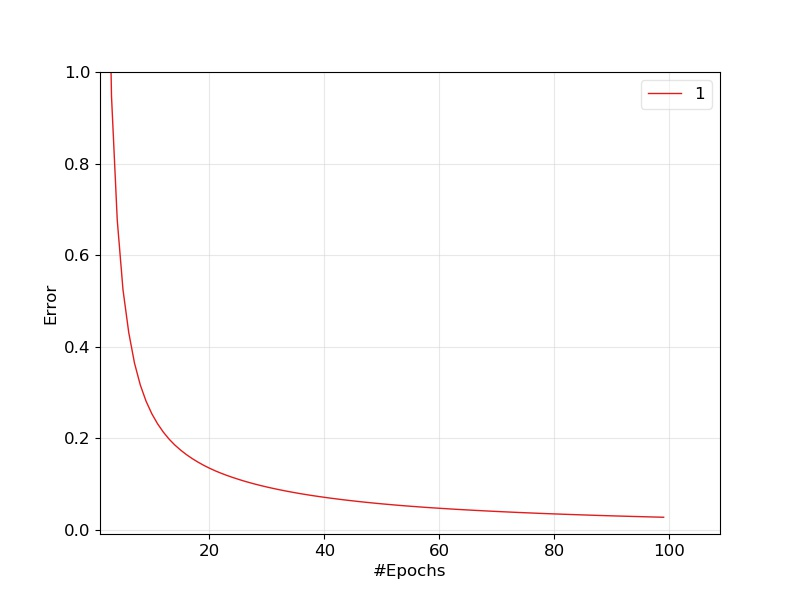
\includegraphics[width=0.8\textwidth]{scripts/one_learning_curve.jpg}


\end{frame}
%----------------------------------------------------------------------
%----------------------------------------------------------------------
\begin{frame}[c]{$10$ Learning Curves  (Setting 1)}

\centering
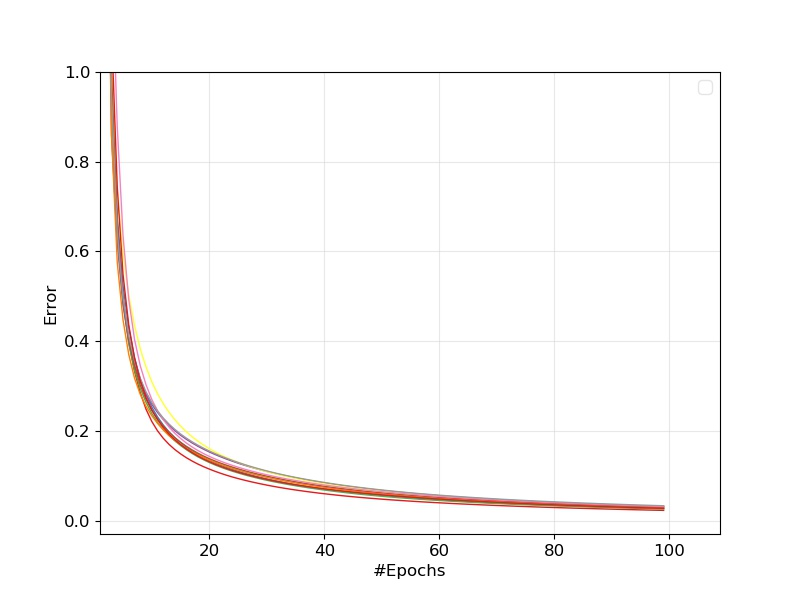
\includegraphics[width=0.6\textwidth]{scripts/ten_learning_curves.jpg}

\begin{itemize}
	\item[$\leadsto$] Deep learning (and most other ML algorithms) are non-deterministc
	\item[$\leadsto$] Measure performance more than once and estimate noise-level
\end{itemize}


\end{frame}
%----------------------------------------------------------------------
%----------------------------------------------------------------------
\begin{frame}[c]{Aggregated Learning Curves (Setting 1)}

\centering
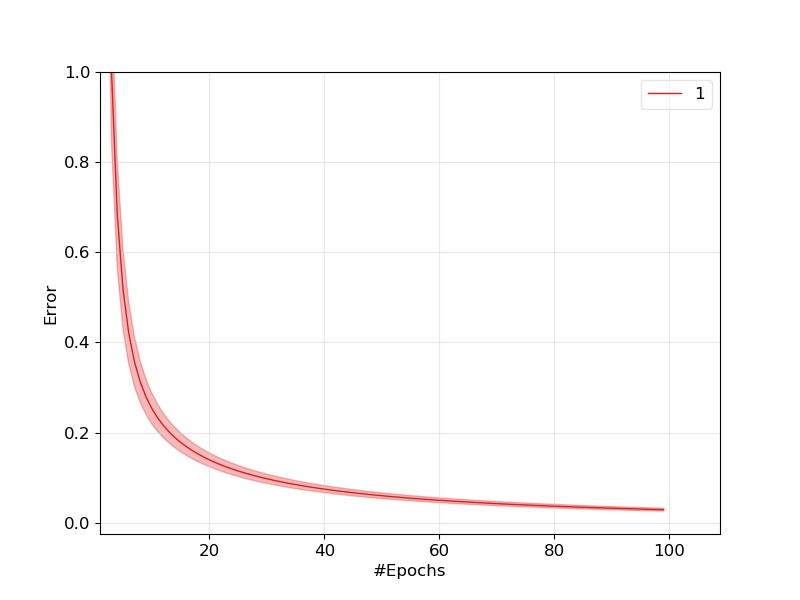
\includegraphics[width=0.6\textwidth]{scripts/hundred_agg_learning_curves.jpg}

\begin{itemize}
	\item Plot mean and stdev (shaded area) across $n$ (here $100$) random seeds\\
	\item Only use mean and stdev
	if noise is somehow normal distributed
	\item alternatives are the mean+standard error or median+25/75-percentiles
\end{itemize}

\end{frame}
%----------------------------------------------------------------------
%----------------------------------------------------------------------
\begin{frame}[c]{Comparing Learning Curves}

\centering
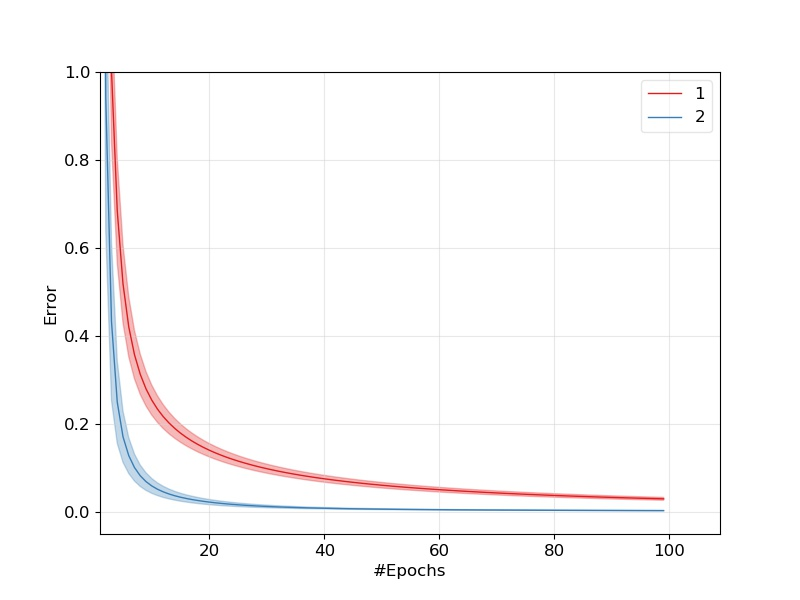
\includegraphics[width=0.7\textwidth]{scripts/compare_learning_curves.jpg}

\begin{itemize}
	\item If uncertainties (shaded area) overlap, results might not be statistically significant but due to noise
\end{itemize}

\end{frame}
%----------------------------------------------------------------------
%----------------------------------------------------------------------
\begin{frame}[c]{Scatter Plot: Train vs. Test}


\begin{columns}
	
\column{0.5\textwidth}

\centering
Setting 1
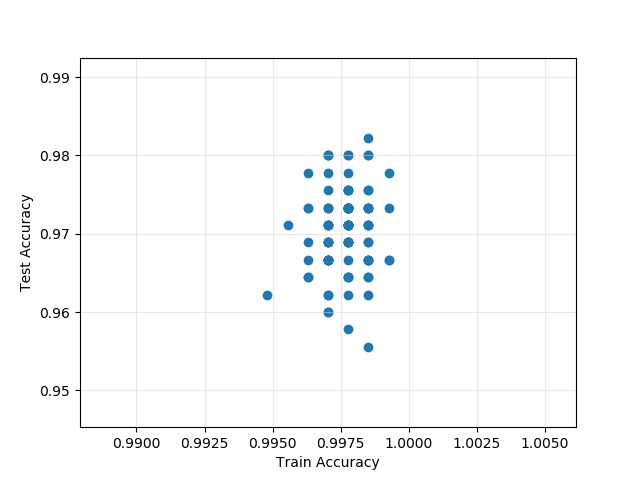
\includegraphics[width=1\textwidth]{scripts/mlp1_test_train_scatter.jpg}

\begin{itemize}
	\item perfect would be if train and test score are correlated
	\item here at least not anti-correlated
\end{itemize}


\column{0.5\textwidth}

\pause
\centering
Setting 2
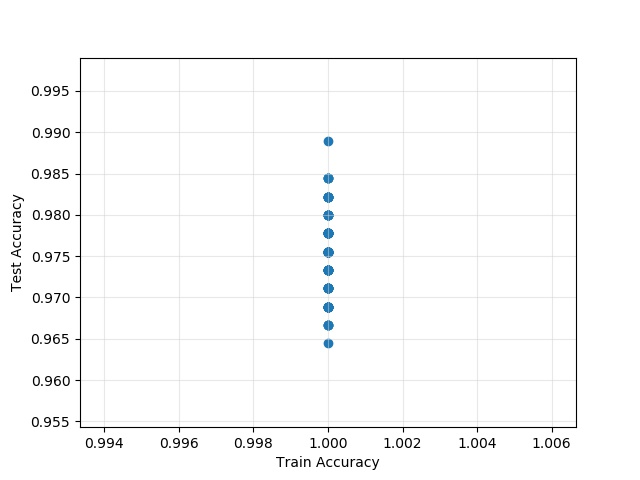
\includegraphics[width=1\textwidth]{scripts/mlp2_test_train_scatter.jpg}
	
\begin{itemize}
	\item already perfect training score
	\item generalization nevertheless noisy
\end{itemize}
	
\end{columns}
	
\end{frame}
%----------------------------------------------------------------------
%----------------------------------------------------------------------
\begin{frame}[c]{eCDF: Distribution of Performance (Setting 1)}

\centering
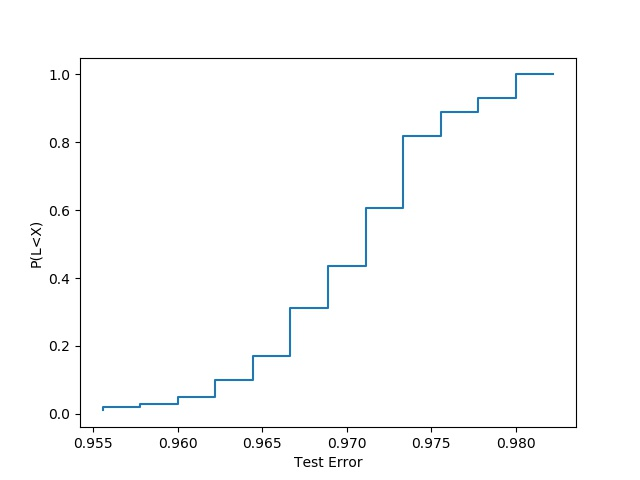
\includegraphics[width=0.6\textwidth]{scripts/mlp1_test_ecdf.jpg}

\begin{flushleft}
	How to compute an empirical CDF:
	\begin{enumerate}
		\item X: sorted error scores
		\item Y: $[1\ldots\#\text{points}] / \#\text{points}$
		\item step\_function(X,Y)
	\end{enumerate}
\end{flushleft}


\end{frame}
%----------------------------------------------------------------------
%----------------------------------------------------------------------
\begin{frame}[c]{eCDF: Distribution of Performance}

\centering
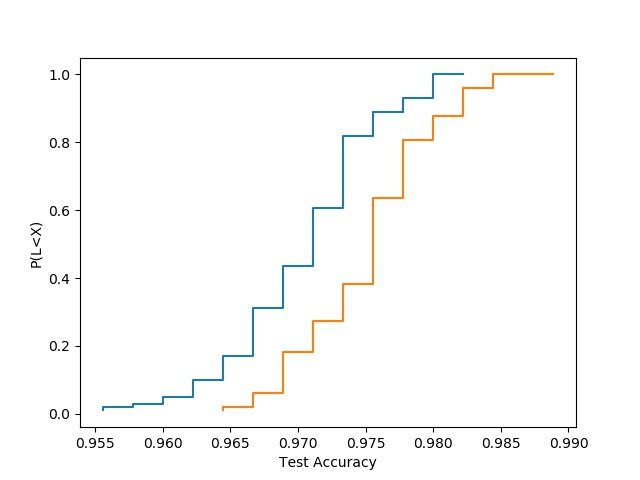
\includegraphics[width=0.6\textwidth]{scripts/mlp12_test_ecdf.jpg}


Which curve corresponds to which setting? \hands

\end{frame}
%----------------------------------------------------------------------
%----------------------------------------------------------------------
\begin{frame}[c]{Box Plot: Comparing Two Configurations}

\centering
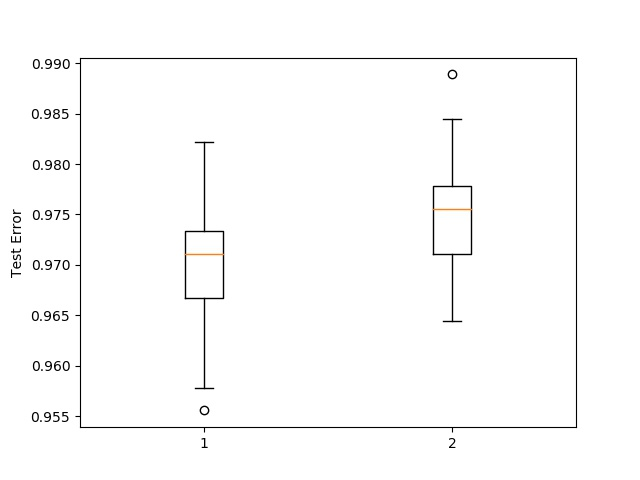
\includegraphics[width=0.6\textwidth]{scripts/mlp12_boxplot.jpg}

\begin{itemize}
	\item alternative: violin plots
	\pause
	\smallskip
	\item if you have paired populations (e.g., configurations evaluated on different datasets),
			you should generate boxplots with $\loss / \loss_{\text{baseline}}$ 
	\item[$\leadsto$] insight on how many datasets one of the two performed better
\end{itemize}
	

\end{frame}
%----------------------------------------------------------------------
%-----------------------------------------------------------------------
\section{Visualization of AutoML Performance}
%----------------------------------------------------------------------
%----------------------------------------------------------------------
\begin{frame}[c]{AutoML Systems over Time}

\begin{itemize}
	\item Don't only measure the performance of AutoML systems for a fixed budget because:
	\begin{enumerate}
	   \item A priori, it is unknown how long a user will run an AutoML system
	   \item Some systems perform well for small budgets and some others need more time before performing well
	   \begin{itemize}
	   	\item BO-based systems often perform as good as\\ random search in the beginning, but perform very well later on
	   \end{itemize}
    \end{enumerate}
	\pause
	\item[$\leadsto$] AutoML systems should have a good anytime performance
	\pause
	\medskip
	\item Recommendation: plot performance (e.g., error) over time
	\begin{itemize}
		\item Similar to learning curves of DNNs 
	\end{itemize} 
\end{itemize}


\end{frame}
%----------------------------------------------------------------------
%----------------------------------------------------------------------
\begin{frame}[c]{Aggregated AutoML Systems over Time}

\centering
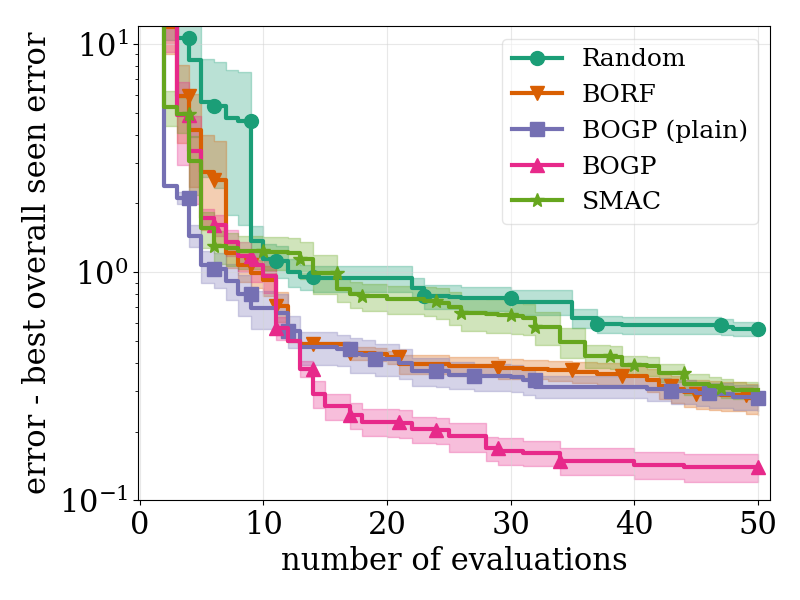
\includegraphics[width=0.5\textwidth]{images/MLPOnMnist_tFalse.png}

\begin{itemize}
	\item Different HPO systems minimizing the error of an MLP on MNIST
	\item How to do it:
	\begin{itemize}
		\item Run each systems several times and always log its current incumbent 
		\item Plot mean and stdev for each system after each incumbent update
		\item Use step functions, because linear interpolation would be\\ too optimistic
	\end{itemize}
\end{itemize}

\end{frame}
%----------------------------------------------------------------------
%----------------------------------------------------------------------
\begin{frame}[c]{Aggregated AutoML Systems over Time and Datasets}

\begin{itemize}
	\item An AutoML system should not only perform well on a single dataset but on many datasets
	\item To summarize and compare the performance across a set of datasets,
	we can plot the performance over time and across datasets
	\pause
	\item Ways to do it:
	\begin{enumerate}
		\item Average loss metric (e.g., error) across datasets
		\begin{itemize}
			\item Problem: different scales of errors on different datasets
		\end{itemize}
	    \pause
	    \item Normalize loss metric across datasets,\\
	    e.g., best seen loss relates to a zero cost
	    \begin{itemize}
	    	\item Problem: Minor improvements ($\leq 0.1\%$) might look substantial
	    \end{itemize}
	\end{enumerate}
    \pause
    \item[$\leadsto$] There is no way around that you have some kind of information loss 
\end{itemize}

\end{frame}
%----------------------------------------------------------------------
%----------------------------------------------------------------------
\begin{frame}[c]{Ranked AutoML Systems over Time and Datasets}


\centering
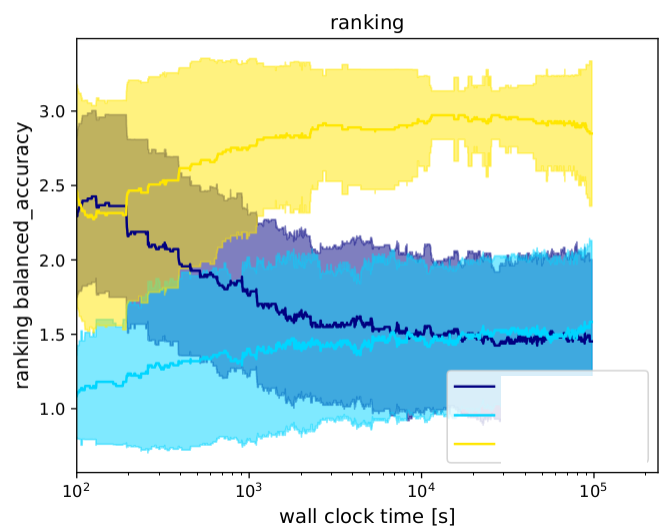
\includegraphics[width=0.5\textwidth]{images/rankings_over_time.png}

\begin{itemize}
	\item Remarks:
	\begin{itemize}
		\item x-axis should be on log-scale
		\item uncertainties (shaded areas) can be obtained via bootstrap sampling
	\end{itemize}
    \pause
    \smallskip
	\item Ranks avoid the problem of different scales
	\item Problem: we don't know whether a better ranking relates to a substantial improvement of the actual cost metric
\end{itemize}

\end{frame}
%----------------------------------------------------------------------
%----------------------------------------------------------------------
\begin{frame}[c]{Scatter Plot: Meta Features}

\begin{columns}
	\column{0.5\textwidth}
	
	\centering
	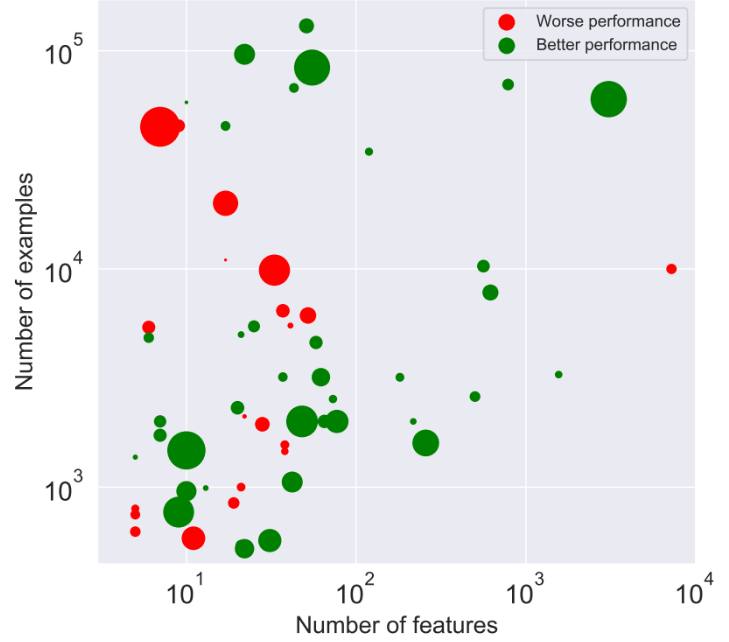
\includegraphics[width=1.0\textwidth]{images/scatter_dataset_twoconfigs.png}
	
	\column{0.5\textwidth}
	\begin{itemize}
		\item Compare two systems\\ (or 1 vs rest)
		\item each dot is a dataset
		\item color encoding better or worse
		\item size indicates performance difference
		\item meta-features (e.g., \#features, \#samples) on axes
		\begin{itemize}
			\item using PCA on a larger set of meta-features leads to algorithm footprints \lit{Smith-Miles et al. 2012}
		\end{itemize}
	\end{itemize}
\end{columns}


\end{frame}
%----------------------------------------------------------------------
%----------------------------------------------------------------------
\begin{frame}[c]{Heatmaps: Comparing several Configurations}

\begin{columns}
	\column{0.5\textwidth}
	
	\centering
	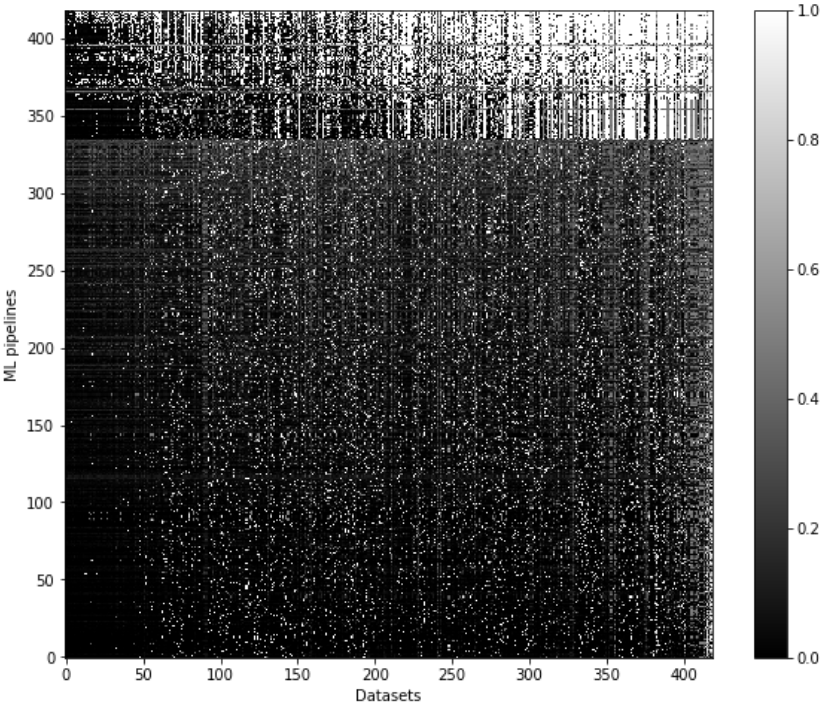
\includegraphics[width=1.0\textwidth]{images/heatmap_pipelines.png}
	
	\column{0.5\textwidth}
	
	\begin{itemize}
		\item compare many configurations on many datasets
		\item can reveal:
		\begin{itemize}
			\item homogeneity if smooth transition from hard to easy
			\item heterogeneity if stripes exist (here the case) 
		\end{itemize}
	    \item Remark: datasets and configurations should be sorted according to their average cost
	\end{itemize}
	
\end{columns}

\end{frame}
%----------------------------------------------------------------------
%-----------------------------------------------------------------------
\section{Statistical Hypothesis Testing}
%----------------------------------------------------------------------
\begin{frame}[c]{Background: statistical hypothesis tests}

\begin{itemize}
	\item When we have a lot of data, we need to summarize it
	\begin{itemize}
		\item But we already saw that summarization hides a lot of data
		%	  \item E.g., a single outlier might explain the difference in means
		\item Ideally, we want to draw high-level conclusions\\
		(e.g., ``A outperforms B on datasets of type X'')
	\end{itemize}
	
	\pause
	\bigskip
	
	\item Problem: we only have a finite number of observations
	\begin{itemize}
		\item Can we attribute observed performance differences to chance?
		\item Are we reasonably sure that a claim we make is reproducible?
		\item[$\leadsto$] Statistical tests can help
	\end{itemize}
	
	
\end{itemize}

\medskip

\end{frame}
%-----------------------------------------------------------------------
%----------------------------------------------------------------------
\begin{frame}[c]{Statistical hypothesis testing}

\begin{enumerate}
\item Define initial research hypothesis
\pause
\item Derive null $H_0$ and alternative $H_1$ hypothesis
\begin{itemize}
	\item Alternative hypothesis should be your research hypothesis
\end{itemize}
\end{enumerate}	

\end{frame}
%-----------------------------------------------------------------------
%----------------------------------------------------------------------
\begin{frame}[c]{First example: Courtroom Tiral}

\begin{itemize}
\item A prosecutor tries to prove the guilt of the defendant
\item $H_0$: 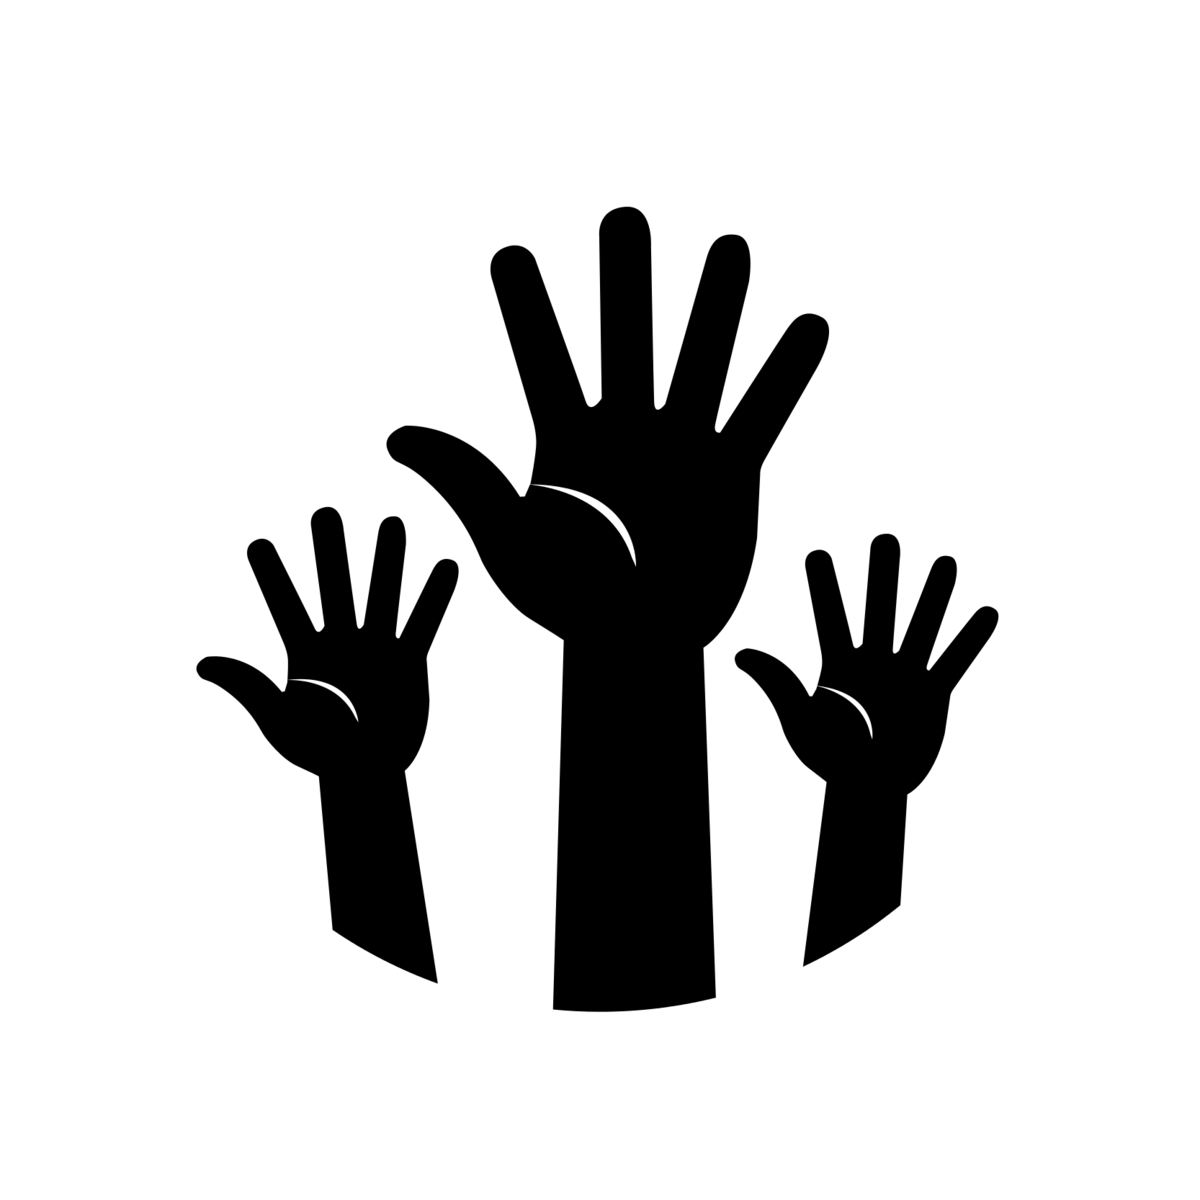
\includegraphics[height=1em]{images/hands} \only<2->{The defendant is not guilty
\begin{itemize}
	\item Accepted for the moment\\ (``not guilty as long as their guilt is not proven'') 
\end{itemize}
}
\item $H_1$: 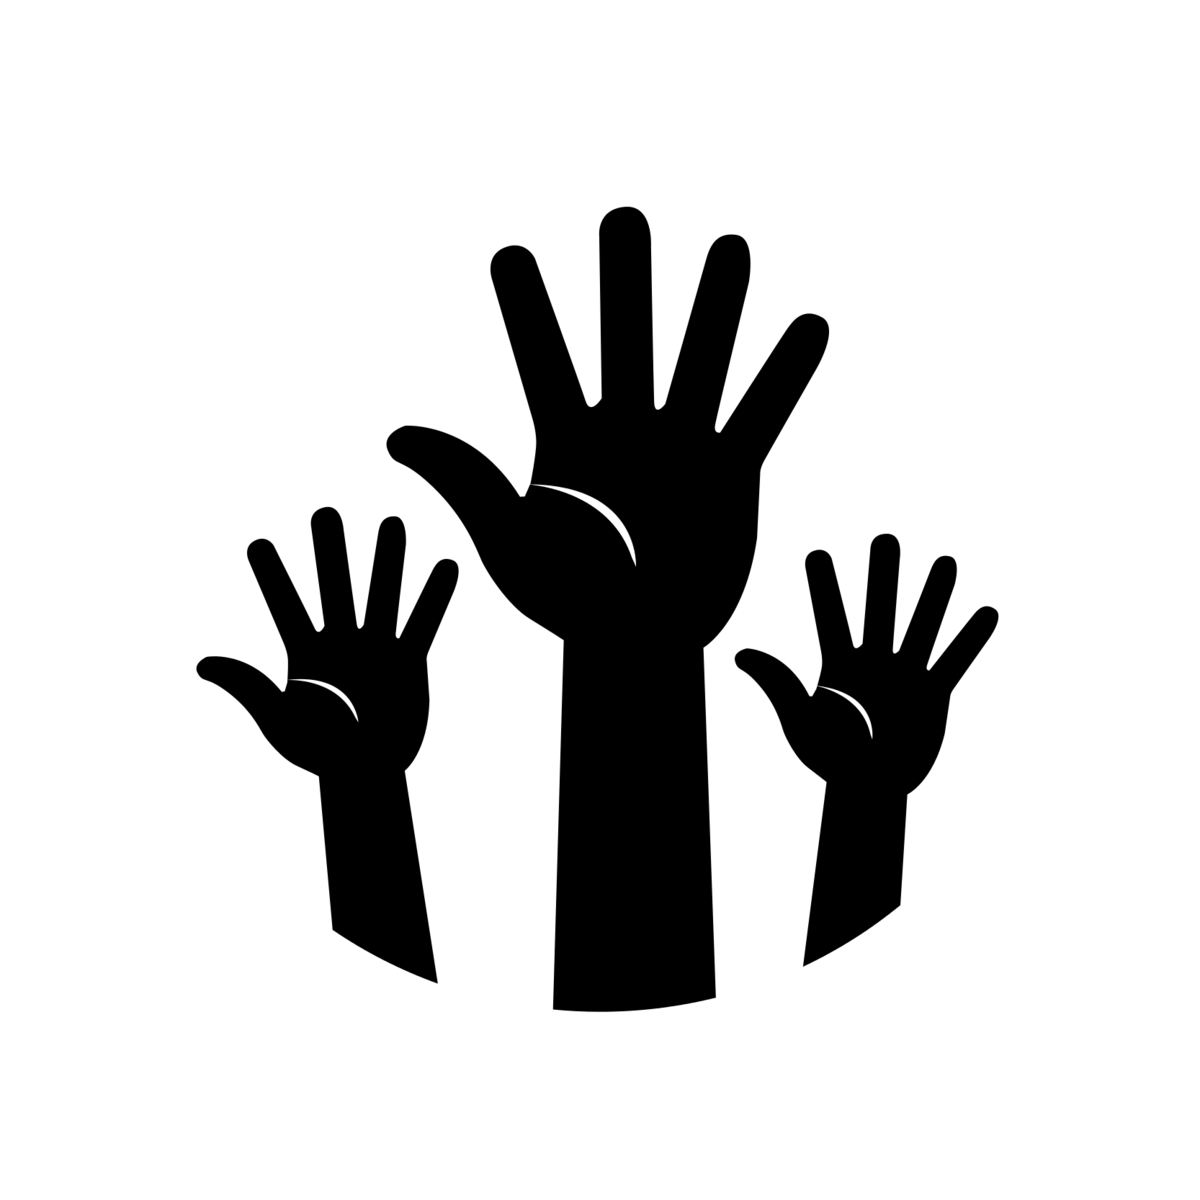
\includegraphics[height=1em]{images/hands} \only<2->{The defendant is guilty
\begin{itemize}
	\item prosecutor hopes to support that
\end{itemize}
}
\pause
\end{itemize}

\medskip
\pause
\bigskip
\centering
\begin{tabular}{r|cc}
\toprule
& Truly not guilty 	& Truly guilty\\
\hline
Found not guilty 	& Acquittal & Type II Error\\
Found guilty & Type I Error		& Conviction\\
\bottomrule
\end{tabular}	

\bigskip
$\leadsto$ We want to minimize Type I error!

\end{frame}
%-----------------------------------------------------------------------
%----------------------------------------------------------------------
\begin{frame}[c]{Statistical hypothesis testing (cont'd)}

\begin{enumerate}
\item Define initial research hypothesis
\item Derive null $H_0$ and alternative $H_1$ hypothesis
\begin{itemize}
\item Alternative hypothesis should be your research hypothesis
\end{itemize}
\item Consider statistical assumptions
\begin{itemize}
\item E.g., is your data Gaussian distributed?
\end{itemize}
\pause
\item Decide test and test statistic $T$
\begin{itemize}
\item The correct test depends on your statistical assumptions.
\item Typically: if you use more assumptions, the test is more powerful\\ (i.e., less Type-I error)
\end{itemize}
\pause
\item Decide significance level $\alpha$\\ (i.e., acceptable Type-I error to reject null hypothesis)
\pause
\item Compute observed $t_{obs}$ of test statistic $T$
\item Calculate $p$-value given $t_{obs}$
\begin{itemize}
\item i.e., probability under the null hypothesis of sampling a test statistic as extreme as observed (probability of Type-I error)
\end{itemize} 
\pause
\item If $p < \alpha$, reject null hypothesis in favor of alternative hypothesis
\begin{itemize}
\item If $p > \alpha$, it doesn't tell you anything about the null hypothesis!
\end{itemize}
\end{enumerate}	

\end{frame}
%-----------------------------------------------------------------------
%----------------------------------------------------------------------
\begin{frame}[c]{Second example for a statistical test}

\begin{itemize}
\item IQ values are known to be normally distributed with $X \sim
\mathcal{N}(100,15)$
\begin{itemize}
\item$\to$ statistical assumption
\end{itemize}
% \\with mean $100$ and variance $15$: $X \sim \mathcal{N}(100,15)$
\item Claim: \alert{``the students in this class are more intelligent
than average''}
\bigskip
\pause
\item \alert{Null Hypothesis $H_0$}: $\mu=100$ ($\mu$ is the population
mean of this class)
\item \alert{Alternative Hypothesis $H_1$}: $\mu>100$ (\alert{one-sided} hypothesis)

\bigskip
\pause

\item Let's say we observed IQ values $x_i$ of 9 students in the class:
\begin{itemize}
\item $\{x_1,\dots,x_9\} = \{116, 128, 125, 119, 89, 99, 105, 116, 118\}$.
\item The \alert{sample mean} is $\bar{x}=112.8$
\item Does this data support the claim?
\end{itemize}	

\end{itemize}	

\end{frame}
%-----------------------------------------------------------------------
%----------------------------------------------------------------------
\begin{frame}[c]{Example continued}

\begin{itemize}

\item \alert{Distribution of the test statistic} 
\begin{itemize}
\item Under $H_0$, we know that each $x_i \sim \mathcal{N}(100,15)$
\smallskip
\item The \alert{test statistic} that we measure is the sample
mean $\bar{x} = \frac{1}{9} \sum_{i=1}^9 x_i$
%    \item[-] $\bar{x} \sim  \mathcal{N}(\mu=100,\sigma^2=15/\sqrt{n})=\mathcal{N}(100,5)$
\bigskip
\pause
\item Under $H_0$, the distribution of $\bar{x}$ is
$\mathcal{N}(100,15/\sqrt{9})$
\begin{itemize}
\item[-] Our observation $\bar{x}=112.8$ is quite extreme under that
distribution
\end{itemize}
\end{itemize}	
\end{itemize}

\begin{center}
%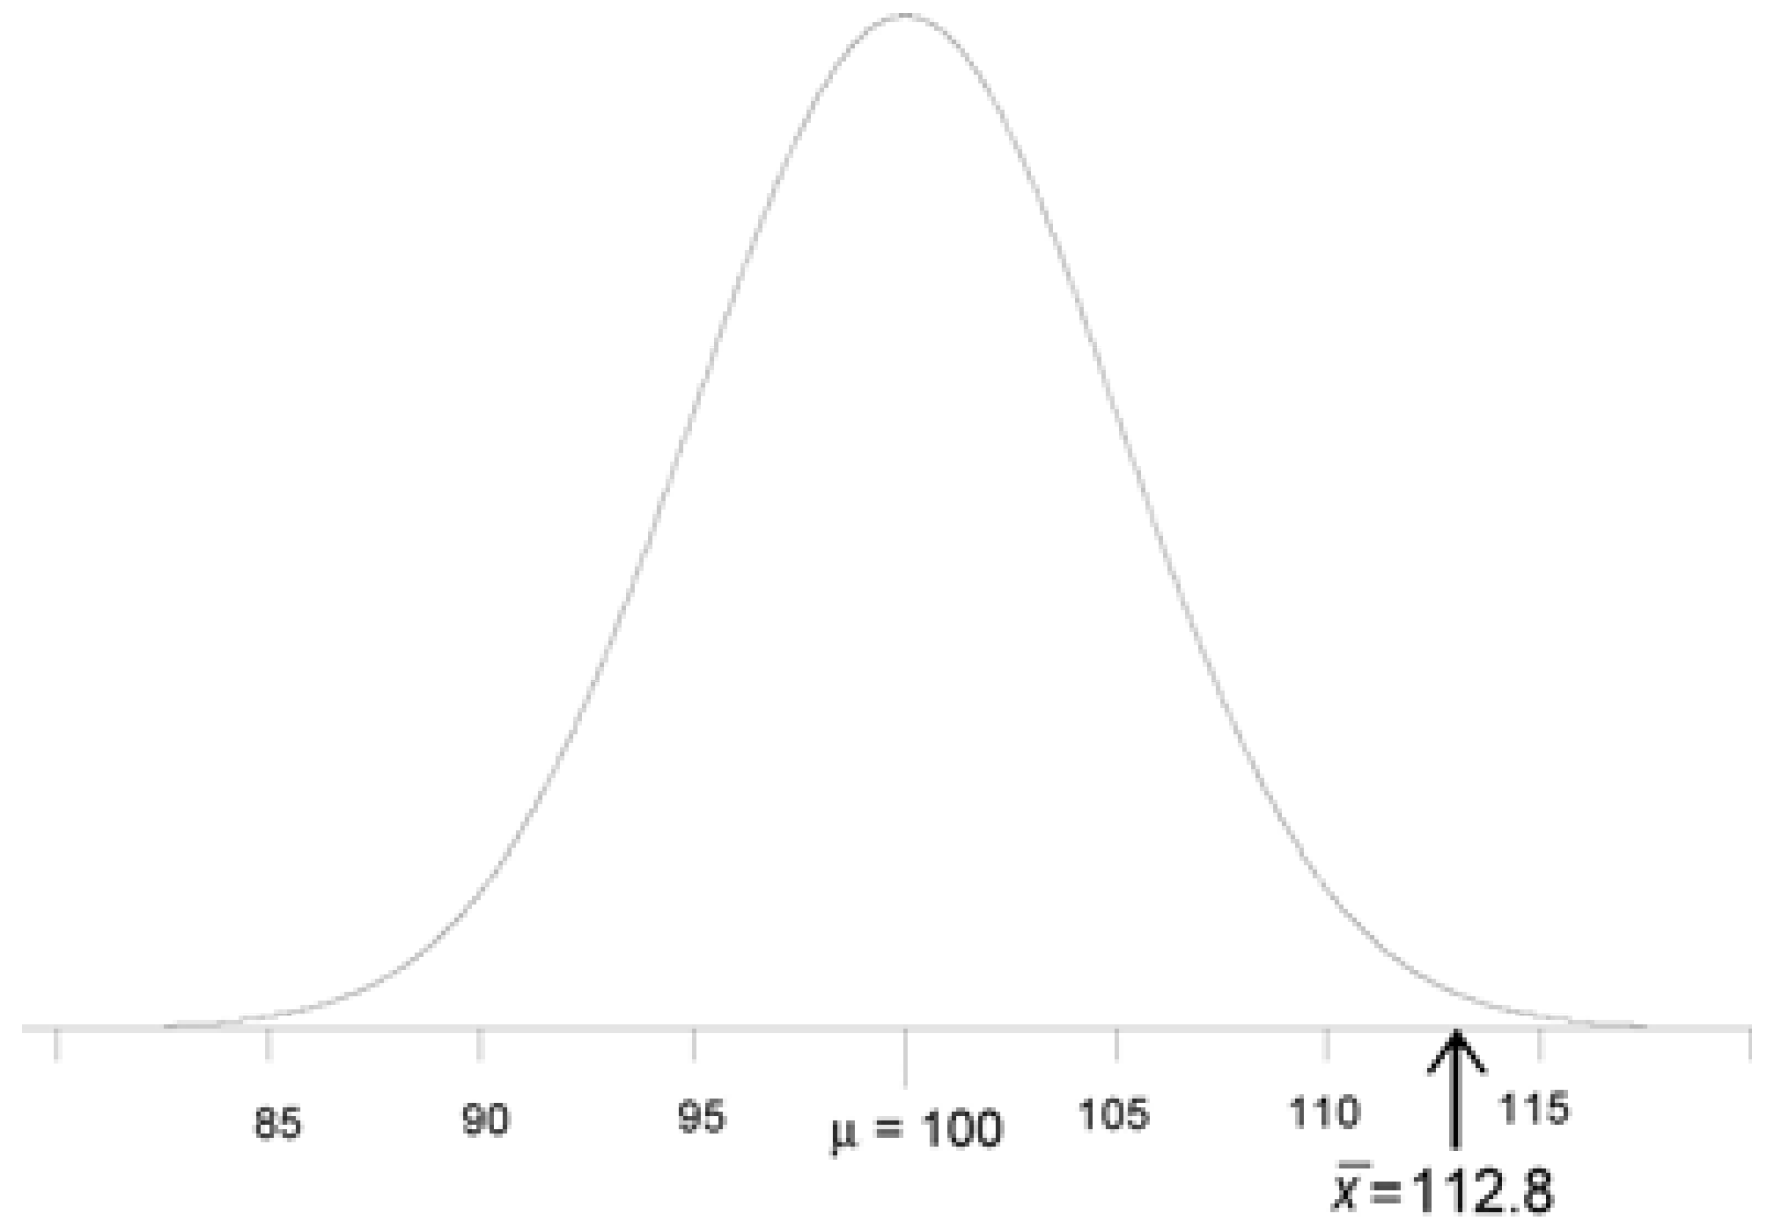
\includegraphics[height=3cm]{images/z_test_1.png}


\pgfmathdeclarefunction{gauss}{2}{%
	\pgfmathparse{1/(#2*sqrt(2*pi))*exp(-((x-#1)^2)/(2*#2^2))}%
}
\tikzstyle{myarrow}=[->, thick]
\begin{tikzpicture}
\begin{axis}[scale=0.75,
no markers, domain=82:118, samples=100,
axis lines*=left, xlabel=$IQ$,axis y line=none,
every axis x label/.style={at=(current axis.right of origin),anchor=west},
every x tick label/.append style={font=\scriptsize, yshift=0.5ex},
height=5cm, width=12cm,label style={font=\tiny},
xtick={80, 85, 90, 95, 100, 105, 110, 115, 120},
xticklabels={$80$, $85$, $90$, $95$, $100$, $105$, $110$, $115$, $120$},
ytick=\empty,
enlargelimits=false, clip=false, axis on top,
x=0.25cm, y=0.25cm/.004,
]
\addplot [thick,cyan!50!black] {gauss(100,15/sqrt(9))};
\coordinate (stat) at (axis cs:112.8,0.00325);
\coordinate (statlabel) at (axis cs:112.8,-.01);
\draw[myarrow, black!75] (statlabel) node [below, font=\scriptsize] {$\bar{x}=112.8$} -- (stat);
\end{axis}

\end{tikzpicture}
\end{center}

\end{frame}
%-----------------------------------------------------------------------
%----------------------------------------------------------------------
\begin{frame}[c]{General principle}

\vspace*{-0.2cm}
\begin{center}
%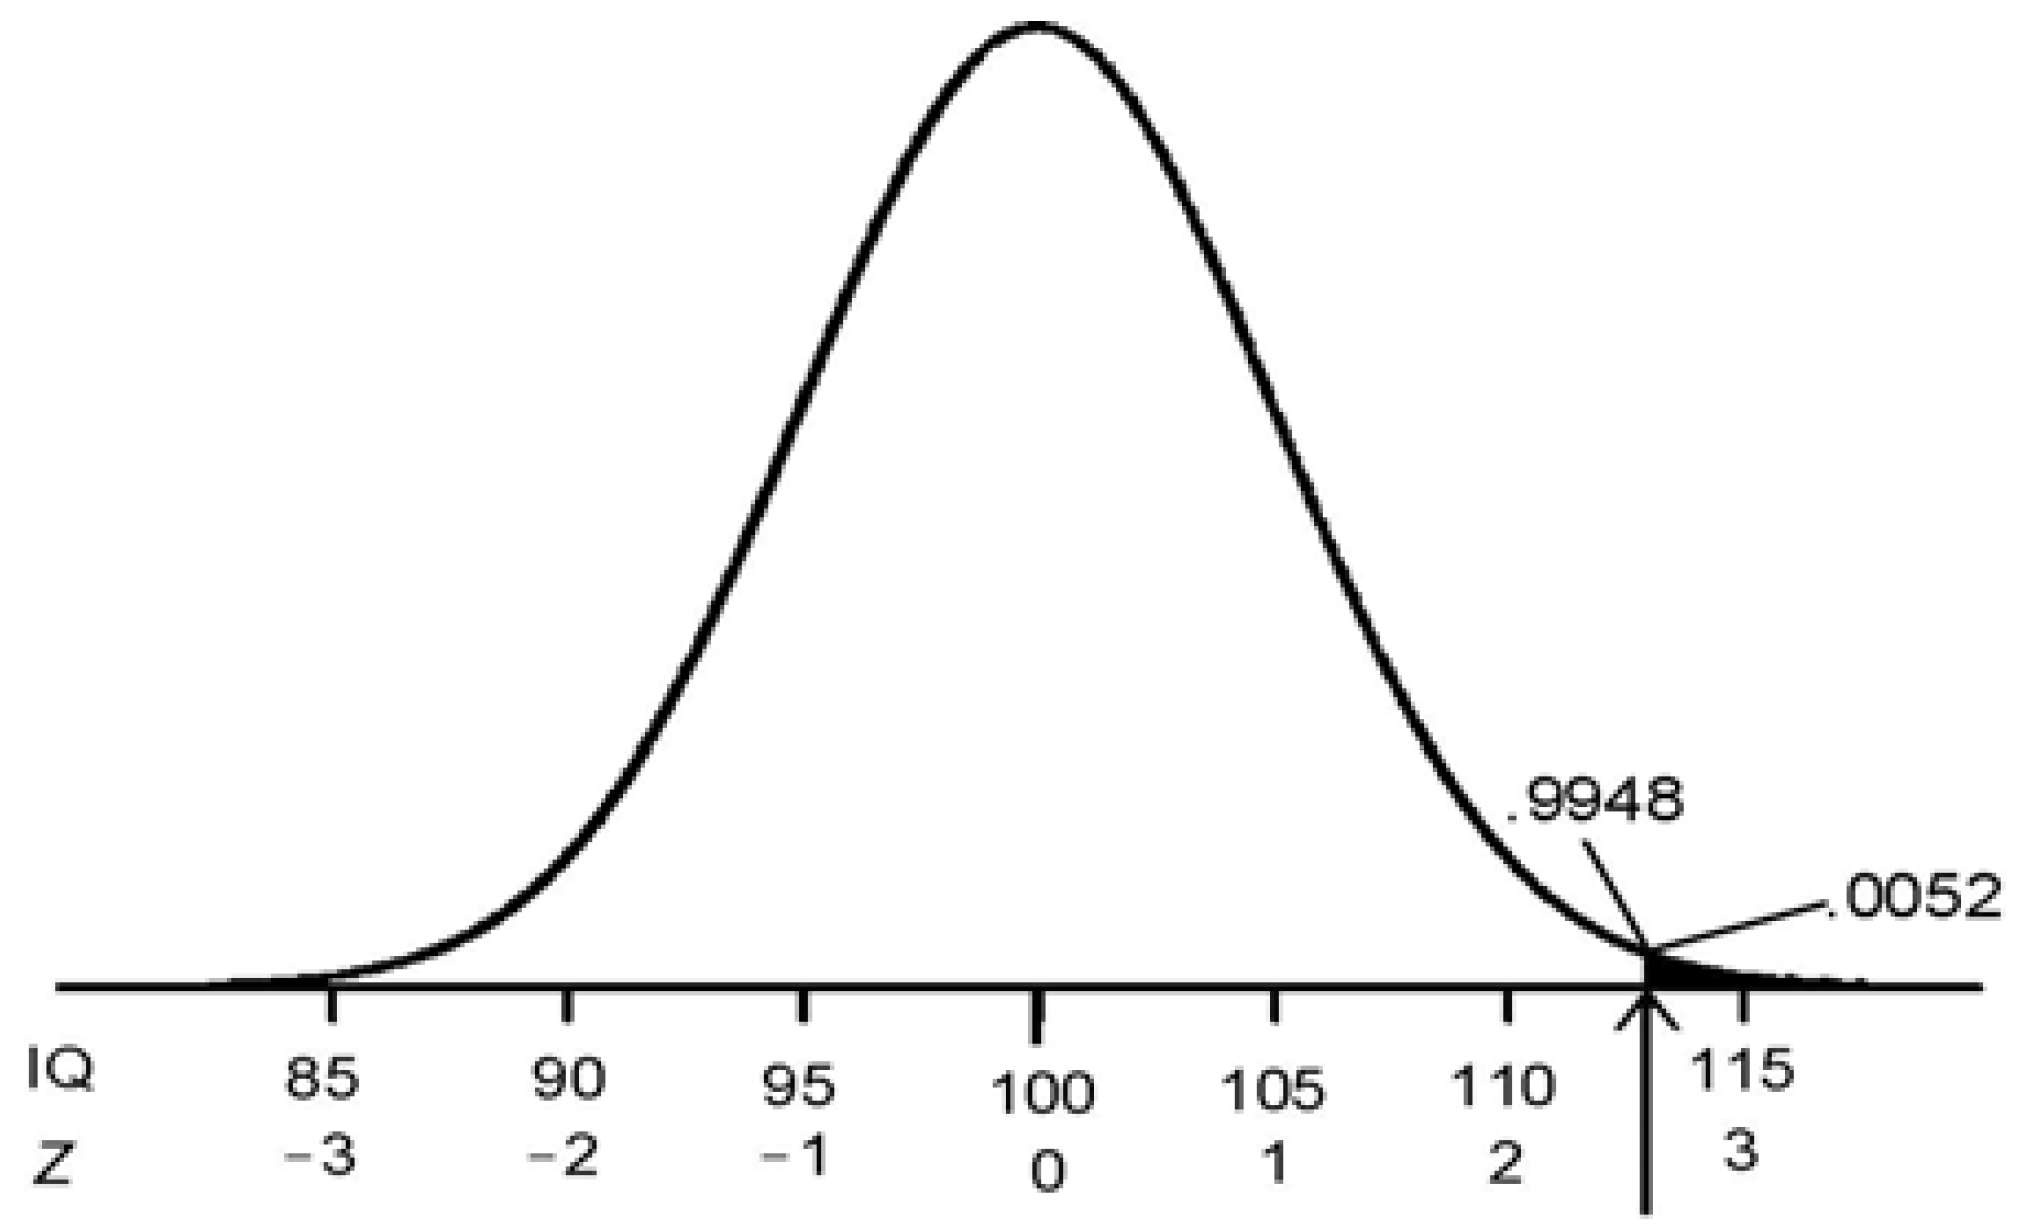
\includegraphics[height=3cm]{images/z_test_2.png}


\pgfmathdeclarefunction{gauss}{2}{%
	\pgfmathparse{1/(#2*sqrt(2*pi))*exp(-((x-#1)^2)/(2*#2^2))}%
}
\tikzstyle{myarrow}=[->, thick]
\begin{tikzpicture}
\begin{axis}[scale=0.525,
no markers, domain=82:118, samples=100,
axis lines*=left, xlabel=$IQ$,axis y line=none,
every axis x label/.style={at=(current axis.right of origin),anchor=west},
every x tick label/.append style={font=\scriptsize, yshift=0.5ex},
height=5cm, width=12cm,label style={font=\tiny},
xtick={80, 85, 90, 95, 100, 105, 110, 115, 120},
xticklabels={$80$, $85$, $90$, $95$, $100$, $105$, $110$, $115$, $120$},
ytick=\empty,
enlargelimits=false, clip=false, axis on top,
x=0.25cm, y=0.25cm/.004,
]
\addplot [fill=black!90, draw=none, domain=112.8:118] {gauss(100,15/sqrt(9))} \closedcycle;
\addplot [fill=black!10, draw=none, domain=82:112.8] {gauss(100,15/sqrt(9))} \closedcycle;
\addplot [thick,cyan!50!black] {gauss(100,15/sqrt(9))};
\coordinate (stat) at (axis cs:112.9,0.0035);
\coordinate (statlabelout) at (axis cs:115,0.0075);
\coordinate (statlabelin) at (axis cs:112,0.0125);
\draw[-, thin] (stat) -- (statlabelout) node[right,font=\tiny]{$.0052$};
\draw[-, thin, black!50] (stat) -- (statlabelin) node[above,font=\tiny]{$.9948$};
\end{axis}

\end{tikzpicture}
\end{center}
\vspace*{-0.2cm}

\begin{itemize}
\item Compare the test statistic (here: $\bar{x}$)\\to its sampling
distribution under $H_0$
\pause 
\medskip
\item \alert{P-value}: probability $p$ of observing values \alert{at least as extreme as $\bar{x}$}\\
%  $\leadsto$ this is the %(computed through cumulative distribution function)
\pause 
\medskip
\item Compare $p$ to pre-defined confidence level $\alpha$ (usually
$\alpha=0.05$);\\\alert{if $p < \alpha$, reject $H_0$}
\pause 
\medskip
\item With $\alpha = 0.01$, would we reject $H_0$ in this case? \hands
\end{itemize}

\end{frame}
%-----------------------------------------------------------------------
%----------------------------------------------------------------------
\begin{frame}[c]{Summary of example}

\begin{itemize}
\item We just used a so-called \alert{$Z$-test}
\item $H_0$: $\mu=\mu_0$, $H_1$: $\mu>\mu_0$  
\item Assumptions: $X \sim \mathcal{N}(\mu,\sigma^2)$ , with known $\mu$ and $\sigma^2$

\medskip
\pause
\item \alert{Test statistic}: sample mean $\bar{x}$; evaluate under 
$\mathcal{N}(\mu=\mu_0,s=\sigma^2/\sqrt{n})$
\pause
\smallskip
\item Equivalent: compute the \alert{Z-statistic}: $Z = (\bar{x}-\mu_0)/s$
and\\
evaluate cumulative distribution $\Phi(Z)$ of $Z$
under $\mathcal{N}(0,1)$
\medskip
\pause
\begin{itemize}
\item There are standard tables to look up $\Phi(Z)$ for different values of $Z$
\item Nowadays, there are standard libraries to compute $\Phi(Z)$
\end{itemize}

\end{itemize}

\end{frame}
%-----------------------------------------------------------------------
%----------------------------------------------------------------------
\begin{frame}[c]{Two-sided tests}


\vspace*{-0.2cm}
\begin{center}
%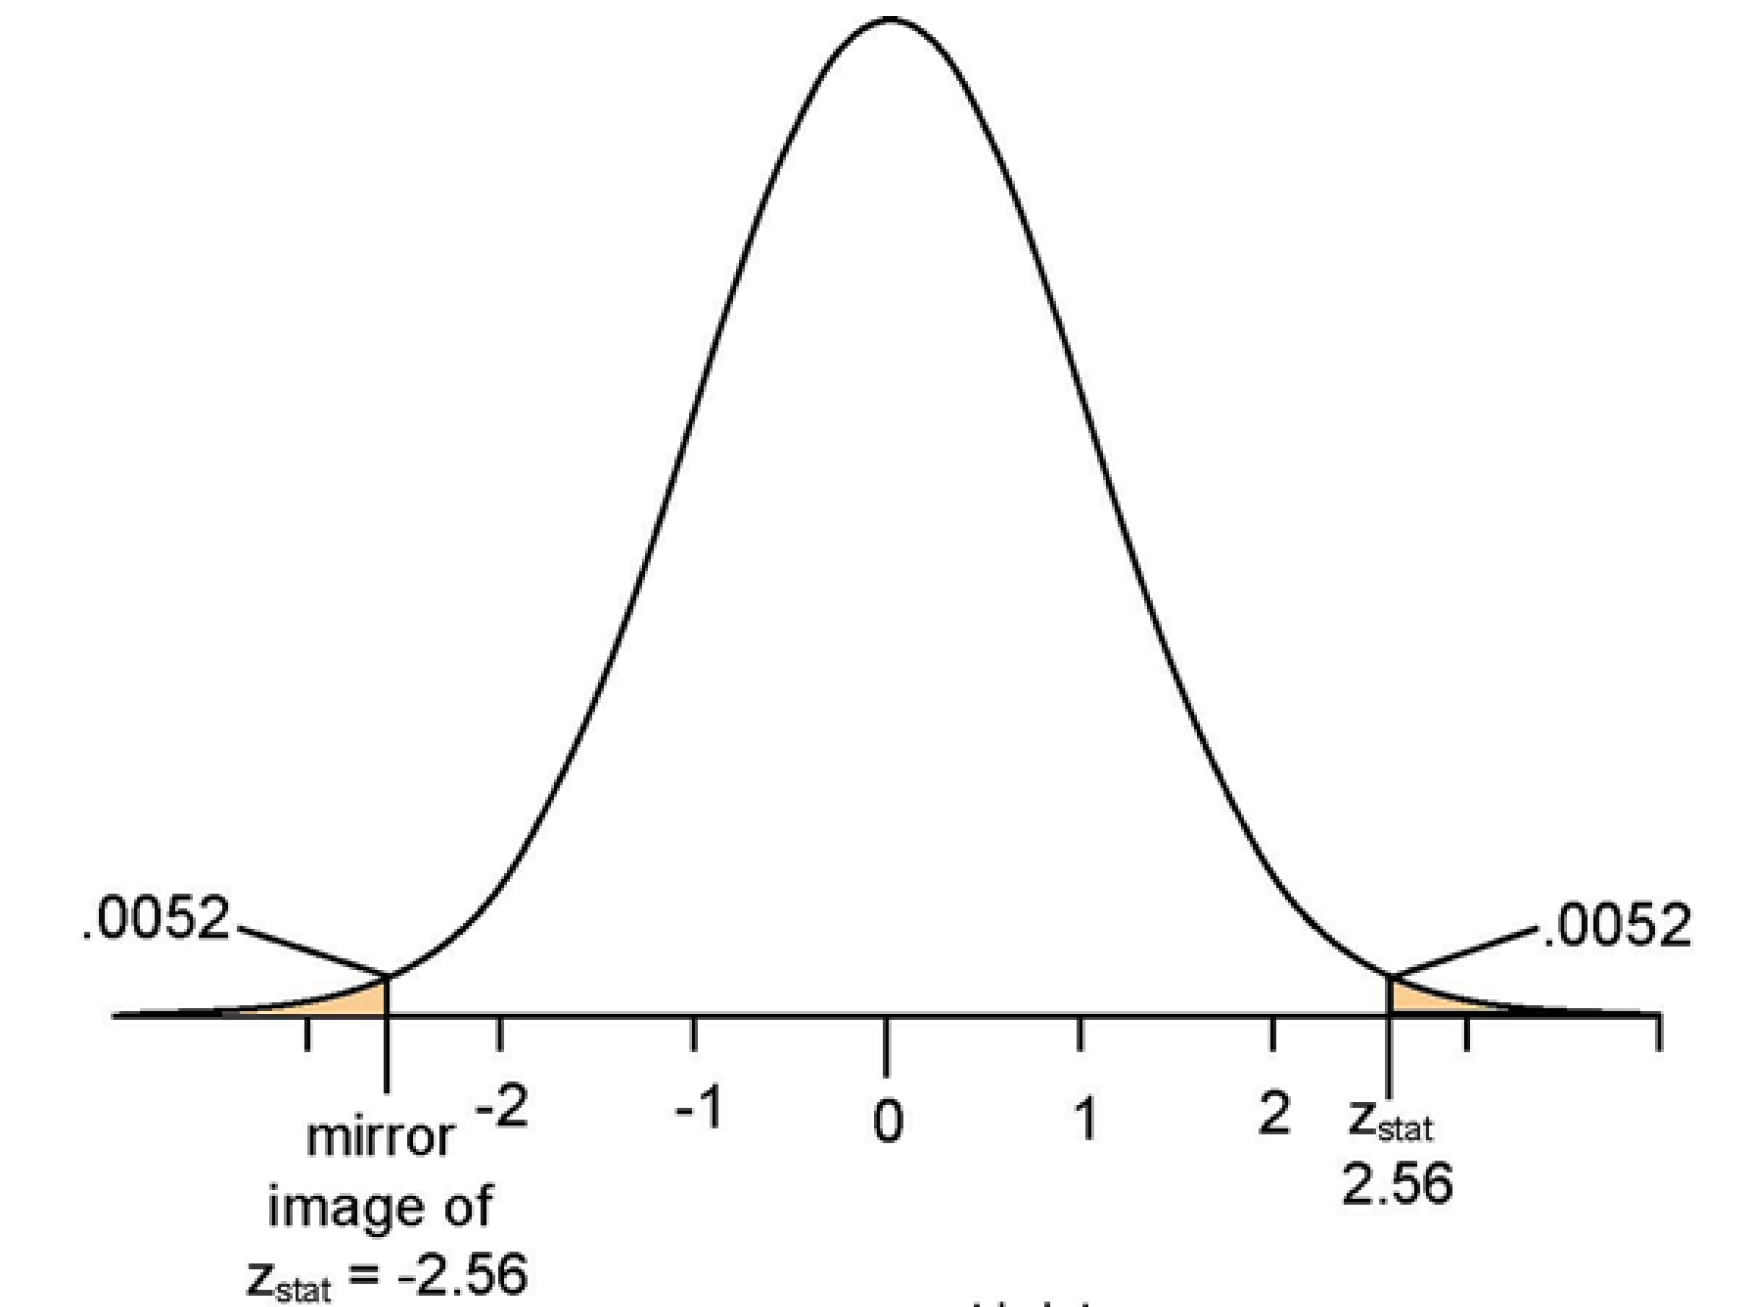
\includegraphics[height=3.5cm]{images/z_test_3.png}


\pgfmathdeclarefunction{gauss}{2}{%
	\pgfmathparse{1/(#2*sqrt(2*pi))*exp(-((x-#1)^2)/(2*#2^2))}%
}
\tikzstyle{myarrow}=[->, thick]
\begin{tikzpicture}
\begin{axis}[scale=0.525,
no markers, domain=82:118, samples=100,
axis lines*=left, xlabel=$IQ$,axis y line=none,
every axis x label/.style={at=(current axis.right of origin),anchor=west},
every x tick label/.append style={font=\scriptsize, yshift=0.5ex},
height=5cm, width=12cm,label style={font=\tiny},
xtick={80, 85, 90, 95, 100, 105, 110, 115, 120},
xticklabels={$80$, $85$, $90$, $95$, $100$, $105$, $110$, $115$, $120$},
ytick=\empty,
enlargelimits=false, clip=false, axis on top,
x=0.25cm, y=0.25cm/.004,
]
\addplot [fill=black!90, draw=none, domain=112.8:118] {gauss(100,15/sqrt(9))} \closedcycle;
\addplot [fill=black!90, draw=none, domain=82:87.2] {gauss(100,15/sqrt(9))} \closedcycle;
%\addplot [fill=black!10, draw=none, domain=82:112.8] {gauss(100,15/sqrt(9))} \closedcycle;
\addplot [thick,cyan!50!black] {gauss(100,15/sqrt(9))};
\coordinate (statright) at (axis cs:112.9,0.0035);
\coordinate (statleft) at (axis cs:87.2,0.0035);
\coordinate (statlabelright) at (axis cs:115,0.0075);
\coordinate (statlabelleft) at (axis cs:85,0.0075);
\draw[-, thin] (statleft) -- (statlabelleft) node[above,font=\tiny]{$.0052$};
\draw[-, thin, black] (statright) -- (statlabelright) node[above,font=\tiny]{$.0052$};
\end{axis}

\end{tikzpicture}
\end{center}
\vspace*{-0.2cm}

\begin{itemize}
\item Similar to one-sided tests, but testing for extreme values in both tails
\item Example Z-test: two-sided alternative hypothesis $H_1$:
$\mu \neq \mu_0$
\pause
\smallskip
\item Compute $Z = (\bar{x}-\mu_0)/s$ as before
\item Compute $p$-value as $p = 2\Phi(Z)$, to account for both tails
\pause 
\medskip
\item With $\alpha = 0.01$, would we reject $H_0$ in this case? \hands
\end{itemize}

\end{frame}
%-----------------------------------------------------------------------
%----------------------------------------------------------------------
\begin{frame}[c]{General points about statistical hypothesis tests}

\begin{itemize}
\item What if $p > \alpha$?
\begin{itemize}
\item \alert{Failure to reject $H_0$}
\item \alert{This does not mean that we accept $H_0$}
\end{itemize}


\pause
\bigskip
\item Beware (i): most tests make some assumptions
\begin{itemize}
\item E.g., $Z$-test and popular $t$-test assume \alert{normality}
\item Our data is often far from normally-distributed
\begin{itemize}
\item[$\leadsto$] E.g., exponential runtime distributions of local search optimizers
\item[$\leadsto$] E.g., distribution of fitting a neural network\\ with different random seeds is not well studied
\end{itemize}
\end{itemize}
\medskip
\pause
\item Beware (ii): if you use cross-validation observations are not independent (you cannot apply statistical tests that assume independence)
%\begin{itemize}
%	\item if you use bootstrap sampling, observations are independent
%\end{itemize}
\end{itemize}

\end{frame}
%-----------------------------------------------------------------------
%----------------------------------------------------------------------
\begin{frame}[c]{The Wilcoxon rank-sum test for non-normal data}

\begin{itemize}
\item Compare the distributions of random variables $X$ and $Y$ 
\begin{itemize}
\item[-] based on samples $x_1, \dots, x_n$ and $y_1, \dots, y_m$
\end{itemize}
\smallskip
\item Assumptions
\begin{itemize}
\item[-] All of $x_1, \dots, x_n$ and $y_1, \dots, y_m$ are independent
from each other 
\item[-] Responses are ordinal (we can compare them)
\end{itemize}  
\pause
\item $H_0$: $P(X > Y) = P(Y > X)$
\pause
\item $H_1$: $P(X > Y) > P(Y > X)$ (one-sided)
\medskip
\pause
\item Test statistic
\begin{itemize}
\item[-] Order all elements $x_i$ and $y_j$ and give them ranks
(1 for smallest)
\item[-] Compute the sum of ranks of $x_i$ and of $y_j$
\smallskip
\pause
\end{itemize}
\item Under $H_0$, the distribution of that test statistic is known\\
$\leadsto$ can evaluate how extreme the observed test statistic is
\end{itemize}

\end{frame}
%-----------------------------------------------------------------------
%----------------------------------------------------------------------
\begin{frame}[c]{The permutation test: another test for non-normal data}

\begin{itemize}
	\item Framework for testing several types of claims
	\item E.g., $H_0$: $X$ and $Y$ have \alert{equal means}
	\item Test statistic: \alert{$t = \frac{1}{n}\sum_{i=1}^n x_i  - 
		\frac{1}{m}\sum_{j=1}^m y_j$}
	\pause
	\medskip
	\item The sampling distribution to compare $t$ against:
	\begin{itemize}
		\item Put $x_1, \dots, x_n$ and $y_1, \dots, y_m$ into a single pool
		\item S = []; repeat, e.g., 10\,000 times
		\begin{itemize}
			\item[-] draw a random permutation \& permute pool with it
			\item[-] add test statistic over permuted pool to $S$
		\end{itemize}
	\end{itemize}
	\pause
	\medskip
	\item $p$-value: percentile of $s$ in $S$:\\
	fraction of samples $s$ in $S$ with $s < t$
	
\end{itemize}

\end{frame}
%-----------------------------------------------------------------------
%----------------------------------------------------------------------
\begin{frame}[c]{Paired vs. unpaired tests}

\begin{itemize}
	\item if you have two unsorted populations (e.g., repeated measurements with different random seeds), you use an unpaired test (as discussed above)
	\item if you can attribute a measurement to concrete objects (e.g., measurements on different datasets), you use a paired test
	\begin{itemize}
		\item paired test are more powerful\\
		(i.e., higher confidence for the same amount of data)
	\end{itemize}
    \item Examples for paired permutation tests
    \begin{itemize}
    	\item Wilcoxon signed rank test
    	\item paired permutation test
    	\begin{itemize}
    		\item permutation of measurement pairs (e.g., same dataset)
    	\end{itemize}
    \end{itemize}
\end{itemize}

\end{frame}
%-----------------------------------------------------------------------
%----------------------------------------------------------------------
\begin{frame}[c]{Multiple Testing Correction}

\begin{itemize}
	\item To compare many systems, we apply statistical tests several time\\
	(once for each pair of systems)
	\item Each test induces some error (bounded by $\alpha$)
	\item[$\leadsto$] the error probability for $k$ tests is bounded by $1 - (1 - \alpha)^k$
	\pause
	\smallskip
	\item Better would be if the error probability would not increase with $k$
	\item[$\leadsto$] multiple testing correction
	\pause
	\smallskip
	\item Bonferronie testing correction: $\alpha_{\text{local}} = \alpha_{\text{global}} / k$
	\pause
	\begin{itemize}
		\item very conservative approach
		\item there exist other, less conservative approaches
	\end{itemize}
	
\end{itemize}

\end{frame}
%-----------------------------------------------------------------------
%----------------------------------------------------------------------
\begin{frame}[c]{Checklist for good scientific practices}

Incomplete list of good scientific practices (specifically for students):
\begin{enumerate}
	\item keep track of your code and design decisions (on all levels)
	\item measure performance of randomized algorithms multiple times\\
		  and show uncertainty of results
	\item apply suitable statistical tests to check for significance
	\item choose a metric that is relevant for the application
	\item always add legends, axis labels and so on in plots
	\item be aware of other research results
	\item avoid peeking at your test data
	\begin{itemize}
		\item no cherry-picking!
	\end{itemize}
\end{enumerate}

\end{frame}
%-----------------------------------------------------------------------
%----------------------------------------------------------------------
\begin{frame}[c]{Learning Goals}

Now, you should be able to \ldots

\begin{itemize}
	\item explain the role of outliers in CS/ML
	\item compare and visualize the performance of different configurations
	\item compare and visualize the performance of AutoML systems
	\item explain and correctly apply statistical hypothesis tests\end{itemize}
\end{frame}
%----------------------------------------------------------------------
%----------------------------------------------------------------------
\begin{frame}[c]{Literature [These are links]}

\begin{itemize}
	\item \lit{\href{https://link.springer.com/content/pdf/10.1023\%2FA\%3A1022623814640.pdf}{P. Langley 1988. Machine Learning as an Experimental Science}}		
    \item \lit{\href{https://www.semanticscholar.org/paper/Machine-Learning-as-an-Experimental-Science-(-)-Drummond/07f052798f17cc761d9e6551c85732e0a41cebb5}{C. Drummod 2006. Machine Learning as an Experimental Science (Revisited)}}	
    \item \lit{\href{http://www.jmlr.org/papers/v7/demsar06a}{J. Demsar 2006. Statistical Comparisons of Classifiers over Multiple Data Sets}}	
    \item \lit{\href{https://journals.plos.org/plosbiology/article?id=10.1371/journal.pbio.1001745}{Wilson et al. 2014. Best Practices for Scientific Computing}}	
    \item \lit{\href{https://journals.plos.org/ploscompbiol/article?id=10.1371/journal.pcbi.1005510}{Wilson et al. 2017. Good enough practices in scientific computing}}
    
    
\end{itemize}

\end{frame}
%----------------------------------------------------------------------
